\subsection{Training}
We train the neural network using Pantheon data, in which the redshift is the feature and the distance module is the target. The pantheon data is split into train and test data in equal size randomly. 512 datapoints are used for training and remaining for testing. The network architecture is described in previous section. We use mean squared error(MSE) loss and Adam\cite{kingma2014adam} optimizer, with early stopping technique to prevent overfitting. Dropout technique with dropout\_rate = 0.2. The hyperparameters used are batch\_size = 10, learning\_rate = 1e-3, patience = 5.
\begin{figure}[H]
	\centering
	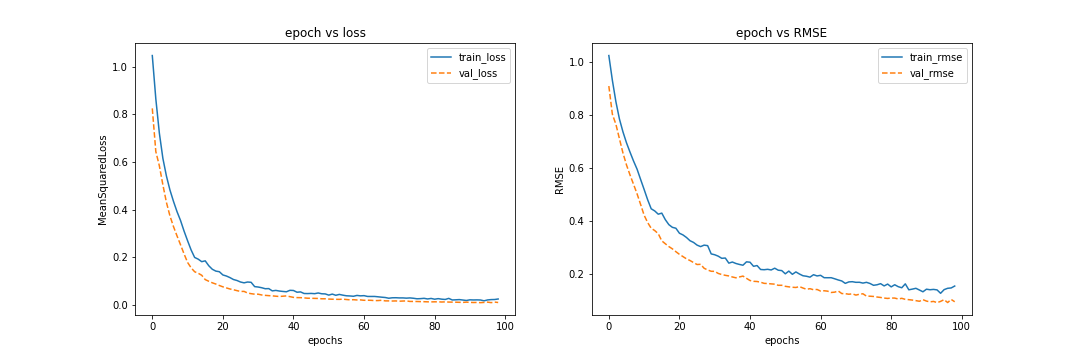
\includegraphics[width=\textwidth]{pantheon/lstm/05_epoch_vs_loss.png}
	\caption{Loss curve}
	\label{fig:loss_curve}
\end{figure}
\begin{figure}[H]
	\centering
	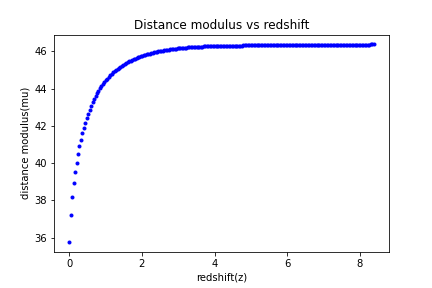
\includegraphics[width=0.8\textwidth]{pantheon/lstm/06_sample_reconstruction.png}
	\caption{Loss curve}
	\label{fig:reconstruction}
\end{figure}